% Brief report style paper

% It's about how a somatotopically ordered pattern can be
% re-established in the cortex based on information carried with
% thalamocortical axons afferent from the ventrobasal thalamus, but
% without specifying absolute positions as center-points for the
% barrels. Everything in the paper should be tailored towards arguing
% this idea.

\documentclass[9pt,lineno]{elife}

\usepackage{color}
\usepackage{amsmath,esint}

% Some document-defined commands
\newcommand*\dif{\mathop{}\!\mathrm{d}}

\input{sebcolour.tex}

% Miscellaneous changes
\newcommand{\cmnt}[1]{\textcolor{colcmnt}{#1}}
% Justify gamma/interaction parameter choice. major point 1.
\newcommand{\MPone}[1]{\textcolor{colmpone}{#1}}
% Blue changes are major point 2 (competition mechanism) and other, general
% uncategorised changes.
\newcommand{\MPtwo}[1]{\textcolor{colmptwo}{#1}}
% Parameter search. Major point 3
\newcommand{\MPthreePar}[1]{\textcolor{colmpthreepar}{#1}}
% Sensitivity analysis. Major point 3
\newcommand{\MPthreeSens}[1]{\textcolor{colmpthreesens}{#1}}
% More predictions. Major point 3
\newcommand{\MPthreePred}[1]{\textcolor{colmpthreepred}{#1}}
% Justify competition:
\newcommand{\mpfive}[1]{\textcolor{colmpfive}{#1}}
% Minor point 4:
\newcommand{\mpfour}[1]{\textcolor{colmpfour}{#1}}
% Minor point 6:
\newcommand{\mpsix}[1]{\textcolor{colmpsix}{#1}}
% Describe the metrics
\newcommand{\metrics}[1]{\textcolor{colmetrics}{#1}}

\newcommand{\dvrg}{\nabla\vcdot\nabla}
\newcommand{\e}{\emph}
\newcommand{\bol}{\textbf}
\newcommand{\mb}[1]{\mathbf{#1}}
\makeatletter
\newcommand*\vcdot{\mathpalette\vcdot@{.35}}
\newcommand*\vcdot@[2]{\mathbin{\vcenter{\hbox{\scalebox{#2}{$\m@th#1\bullet$}}}}}
\newcommand{\code}[1]{\textsf{#1}}
% Nice norms:
\usepackage{mathtools}
\DeclarePairedDelimiter{\norm}{\lVert}{\rVert}
% Degrees symbol:
\usepackage{textcomp}

\title{Modelling the emergence of whisker barrels}

\author[1*]{Sebastian~S.~James}
\author[2]{Leah~A.~Krubitzer}
\author[1]{Stuart~P.~Wilson}

\affil[1]{Department of Psychology, The University of Sheffield, Sheffield, United Kingdom.}
\affil[2]{Center for Neuroscience, The University of California, Davis, United States.}
\corr{seb.james@sheffield.ac.uk}{SSJ}

%\keywords{Barrel cortex $|$ Self-organization $|$ Somatotopic map $|$ Axon guidance}

\begin{document}

\maketitle

\begin{abstract}
Brain development relies on an interplay between genetic specification and
self-organization. Striking examples of this relationship can be found in the
somatosensory brainstem, thalamus, and cortex of rats and mice, where the
arrangement of the facial whiskers is preserved in the arrangement of cell
aggregates to form precise somatotopic maps. We show in simulation how
realistic whisker maps can self-organize, by assuming that information is
exchanged between adjacent cells only, under the guidance of gene expression
gradients. The resulting model provides a simple account of how patterns of
gene expression can constrain spontaneous pattern formation to faithfully
reproduce functional maps in subsequent brain structures.
\end{abstract}

\section{Introduction}

Spatial patterns in neural connectivity provide clues about the constraints
under which brains evolve and develop \citep{purves_iterated_1992}. Perhaps
the most distinctive pattern can be found in the barrel cortex of many rodent
species \citep{woolsey_structural_1970}. The barrels are identifiable soon
after birth in layer 4 of primary somatosensory cortex as dense clusters of
thalamocortical axons, which are enclosed by borders a few neurons thick from
postnatal day 3 \citep{erzurumlu_development_2012}.
%
% These timings, from erzurumlu_development_2012 originate from
% sehara_neuronal_2011, where they relate to mouse.
\mpsix{In the mouse, axons from the trigeminal ganglion arrive in the principal sensory
  nucleus of the trigeminal nerve (PrV) at E12, then axons from the PrV arrive
  in the ventroposteromedial nucleus of the thalamus (VPM) at E17, then axons
  from the VPM arrive in the cortical plate at E18/P0. Distinct whisker-related
  clusters then become apparent in the PrV at P0-P1, in the VPM at P2-P3, and
  in the cortex at P3-P5} \citep{erzurumlu_development_2012,sehara_neuronal_2011}.
%
In the plane tangential to
the cortical surface the barrels constitute a somatotopic map of the whiskers,
with cells within adjacent barrels responding most strongly and quickly to
deflection of adjacent whiskers \citep{armstrong-james_flow_1992}. Barrel
patterning reflects subcortical whisker maps comprising cell aggregates called
barrelettes in the brainstem and barreloids in the thalamus
\citep{ma_barrelettesarchitectonic_1991,van_der_loos_barreloids_1976}.

Barrel formation requires afferent input from whisker stimulation and thalamic
calcium waves \citep{anton-bolanos_prenatal_2019}, and depends on a complex
network of axon guidance molecules such as ephrin-A5 and A7 and adhesion
molecules such as cadherin-6 and 8
\citep{vanderhaeghen_mapping_2000,miller_epha7-ephrin-a5_2006}.  This network
is orchestrated by interactions between morphogens Fgf8 and Fgf17 and
transcription factors Emx2, Pax6, Sp8, and Coup-tf1
\citep{shimogori_fibroblast_2005,bishop_regulation_2000}, which are expressed
in gradients \mpfour{across the full cortical sheet} that mark orthogonal axes
and can be manipulated to stretch,
shrink, shift, and even duplicate barrels
\citep{assimacopoulos_fibroblast_2012}.

The barrel boundaries form a Voronoi tessellation across the cortical sheet
\citep{senft_mouse_1991} (Fig.\,\ref{fig:main}A), suggesting that barreloid topology is
preserved in the projection of thalamocortical axons into the cortex, and that
a barrel forms by lateral axon branching from an initial center-point that
ceases upon contact with axons branching from adjacent centers.  However, the
assumption of pre-arranged center-points is difficult to resolve with the
observation that axons arrive in the cortical plate as an undifferentiated
bundle, \emph{prior} to barreloid formation \citep{agmon_organized_1993}.

Alternatively, reaction-diffusion dynamics could generate a Voronoi
tessellation without pre-arranged centers, by amplifying characteristic modes
in a noisy initial distribution of axon branches, as a net effect of
short-range cooperative and longer-range competitive
interactions. Accordingly, the barrel pattern would be determined by the
relative strength of these interactions and by the shape of the cortical field
boundary. However, intrinsic cortical dynamics alone cannot account for the
topographic correspondence between thalamic and cortical domains, the
irregular sizes and specific arrangement of the barrels in rows and arcs, or
the influence of gene expression gradients.

The center-point and reaction-diffusion models are not mutually
exclusive. Pre-organized centers could bias reaction-diffusion processes to
generate specific arrangements more reliably, and mechanisms of lateral axon
branching may constitute the tension between cooperation and competition
required for self-organization. However, proof that barrel patterning can
emerge from an undifferentiated bundle of axons, based only on local
interactions, would show that a separate stage and/or extrinsic mechanism for
pre-organizing thalamocortical connections need not be assumed. To this end,
we ask whether barrel maps can emerge in a system with reaction-diffusion
dynamics, under the guidance of signalling gradients, and in the absence of
pre-defined centers.

\section{Models}

\cite{karbowski_model_2004} developed a reaction-diffusion style model of how
extrinsic signalling gradients can constrain the emergence of distinct fields
from intrinsic cortical dynamics. Their model defines how the density of
connections $c(x,t)$ and axon branches $a(x,t)$ interact at time $t$, along a
1D anterior-posterior axis $x$, for $N$ thalamocortical projections indexed by
$i$. The model was derived from the assumption that the rates at which $a_i$
and $c_i$ grow are reciprocally coupled. Extending the original 1D model to
simulate arealization on a 2D cortical sheet, we use $a_i(\mb{x},t)$ and
$c_i(\mb{x},t)$, and model synaptogenesis as
%
\begin{equation} \label{eq:dc}
\frac{\partial c_i}{\partial t} =-\alpha c_i +\beta  \left(1 - \sum_{j=1}^{N} c_{j}\right)[a_i]^k.
\end{equation}
%
Accordingly, where the total density of synaptic connections sums to one,
connections decay at rate $\alpha$. Otherwise the connection density increases
non-linearly ($k>1$) with the density of axon branching. Axon branching is
modelled as
%
\begin{equation} \label{eq:da}
\frac{\partial a_i}{\partial t} = \nabla\vcdot\left(D \nabla a_i-a_i\sum_{j=1}^{M} \gamma_{i,j}\nabla \rho_j(\mb{x}) \MPtwo{+ \chi_i}\right) - \frac{\partial c_i}{\partial t}.
\end{equation}
%
The first term on the right describes the divergence (indicated by
$\nabla\vcdot$) of the quantity in parentheses, which is referred to as the
`flux' of axonal branching. The flux represents diffusion across the cortical
sheet, at rate $D$, and the influence of $M$ molecular signalling fields,
$\rho(\mb{x})$. The influence of a given field (indexed by $j$) on a given
thalamic projection (indexed by $i$), is determined by $\gamma_{i,j}$, which
may be positive or negative in order that axons may branch in the direction of
either higher or lower concentrations. Note that computing the divergence in
simulation requires cells on the cortical sheet to communicate with immedately
adjacent cells only (see \emph{Materials \& Methods}). The second term on the
right quantifies the coupling between axon branching and synaptogenesis. Here
  $\chi_i=0$ is a placeholder.

\section{Results}

\begin{figure}
  \begin{fullwidth}
    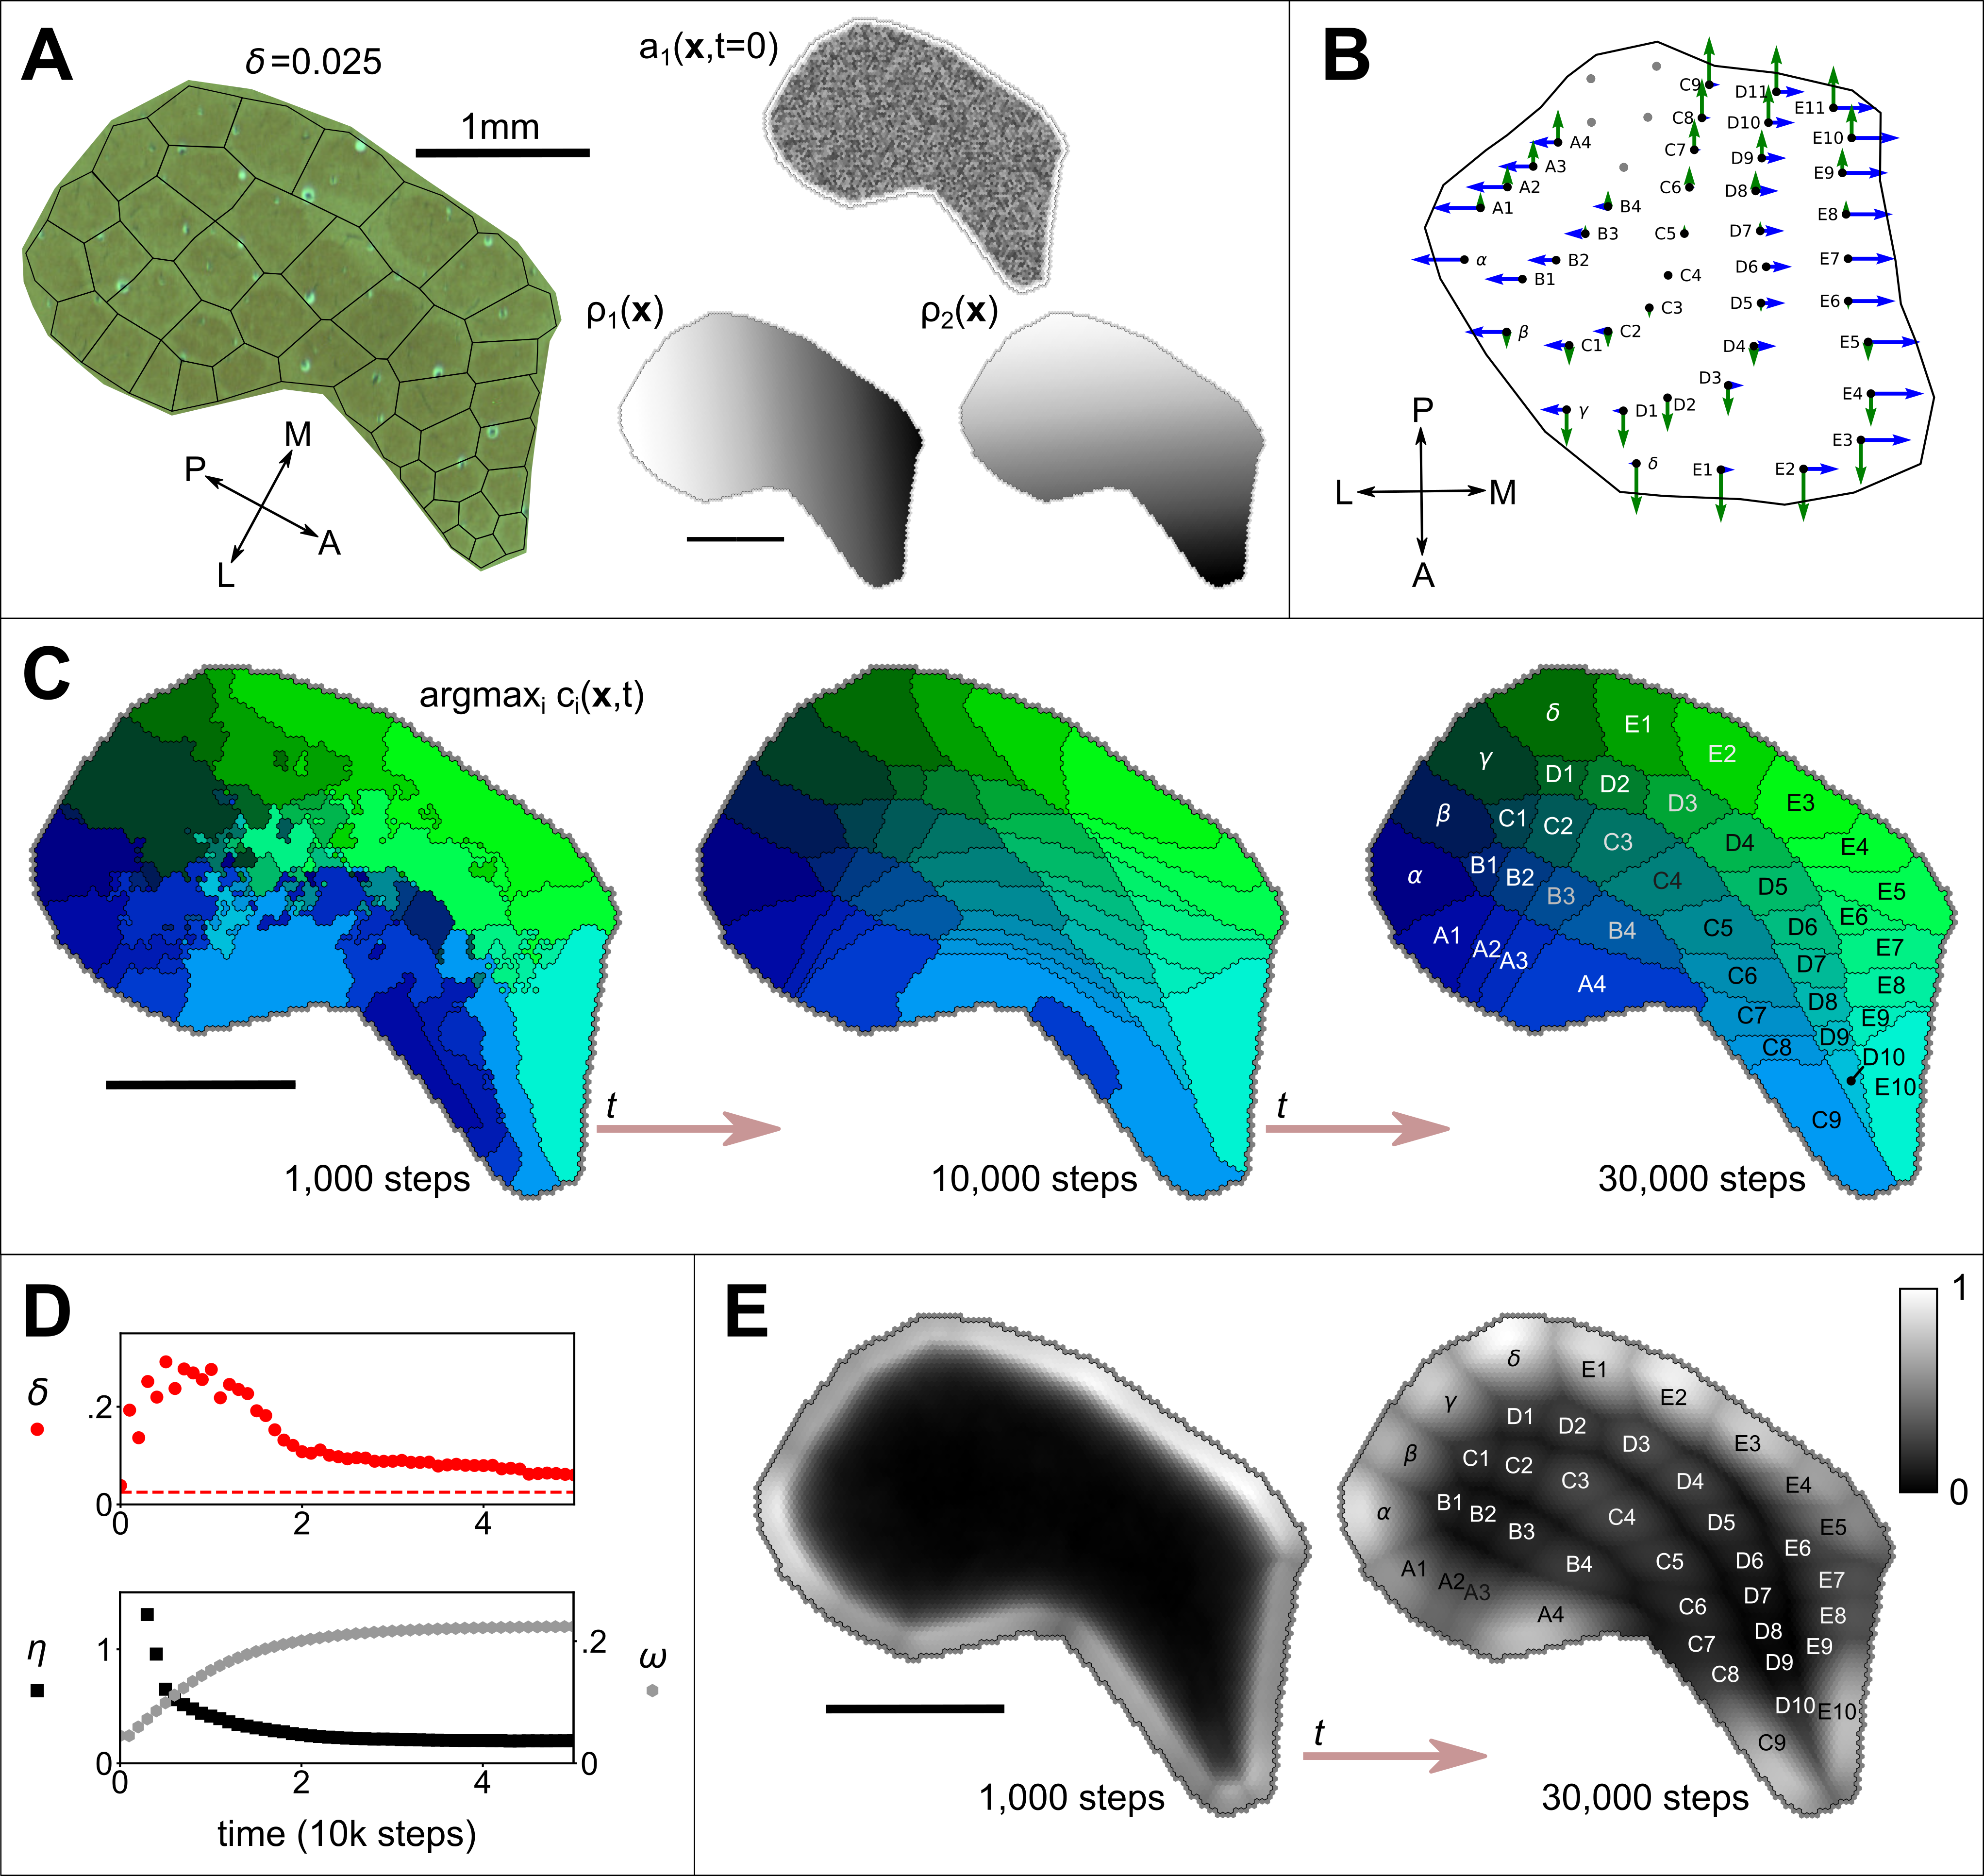
\includegraphics[width=\linewidth]{./Fig1.png}
    \caption{\textbf{A} Left shows a cytochrome oxidase stain obtained from rat S1
      by \cite{zheng_signal_2001}, with black lines to delineate barrels and to
      measure departure (Honda-$\delta$; see \citealp{senft_mouse_1991}) from a
      perfect Voronoi tesselation. Right shows the initial distribution of axon
      branching density ($a$) for one thalamocortical projection, and two
      molecular guidance fields ($\rho$), \cmnt{where the domain $S$ has been
        traced from \textbf{A}}. \textbf{B} The strengths of interaction
      $\gamma$ with fields $\rho_1$ and $\rho_2$ are indicated for each of 41
      projections by the lengths of green and blue arrows respectively, assuming
      that similar fields aligned to the posterior-anterior and medial-lateral
      axes in the ventroposterior medial nucleus of the thalamus are sampled at
      the locations of putative barreloid centers (reconstructed from
      \citealp{haidarliu_size_2001}, \MPone{Fig.\,5b}). \textbf{C} Simulation results for parameters
      \MPtwo{$N=41$, $\alpha=3.6$, $\beta=16.67$, $k=3$, $D=0.5$, $\gamma\in\pm 2$,
      $\epsilon=1.2$} and $\delta{t}=0.0001$. Colours indicate the thalamic
      projection for which the connection density is maximal and black lines
      delineate boundaries (see Movie
      S1). \textbf{D} Red dots show the Honda metric, \metrics{$\delta(t)$}, obtained from \metrics{the}
      simulation approaching that obtained from \metrics{real} barrels in \textbf{A} (dotted
      line); black squares \metrics{provide a} measure \metrics{of} the correspondence
      between the real and
      simulated barrel shapes, $\eta(t)$ (the \metrics{pattern quality metric---see
        Materials \& Methods; units mm$^3$});
      \metrics{grey hexagons \metrics{provide a measure of how selectively each
          cortical site is innervated};
        $\omega(t) = \oiint_{S} \mu(\mb{x},t) \mathrm{d}S$, where
        $\mu(\mb{x}) \equiv \mathrm{max}_i\big(c_i(\mb{x},t)\big)\big/\sum_{j=1}^{N} c_j(\mb{x},t)$.}
      \textbf{E} \metrics{Plotted across the cortical sheet, the selectivity
        develops to reveal an alignment with the emergent barrel boundary
        shapes}. \metrics{The colour map
        indicates the values of $\mu(\mb{x})$. Overlaid
        contours show $c_i > 0.95 \mathrm{max}_i\big(c_i(\mb{x})\big)$.} All scale bars 1\,mm.}
    \label{fig:main}
  \end{fullwidth}
\end{figure}

First we verified that all results established by \cite{karbowski_model_2004}
for a 1D axis could be reproduced using our extension to a 2D cortical
sheet. Using an elliptical domain, $S$, with $M=3$ offset guidance gradients
aligned to the longer axis, $N=5$ thalamocortical projections gave rise to
five distinct cortical fields at locations that preserved the topographic
ordering defined by the original $\gamma$ values. However, we found that
specifying $N$ ordered areas required $M\approx (N+1)/2$ signalling
fields. This is because localization of axon densities occurs only when
projections are influenced by interactions with two or more signalling
gradients that encourage migration in opposing directions. As the number of
guidance fields is unlikely to approach the number of individual barrels,
\cmnt{modifications to the model} were required.

\mpfive{We reasoned that an arbitrary number of distinct field locations may
  be specified using a minimum of two guidance fields, if the tendency for the
  density of each projection to concentrate is appropriately balanced against
  the tendency of projections that interact more strongly with the guidance
  fields to migrate further in the directions specified by their
  gradients. Accordingly, projections that interact most strongly with a given
  guidance gradient would come to occupy cortical locations at which that
  field has extreme values, leaving adjacent locations available to be
  occupied by projections with the next strongest interactions, and so
  forth. This would in principle allow the \emph{relative} locations of the
  fields to be specified by the relative values of the interaction parameters,
  $\gamma$, and hence for a topological map in the cortex to be specified by a
  spatial ordering of the $\gamma$ values at the level of the thalamus.}

\mpfive{Such dynamics are quite unlike those described by classic
  chemospecificity models} \citep{sperry_chemoaffinity_1963}, \mpfive{which
  essentially assume center-points by specifying conditions in the target
  tissue that instruct pre-identified afferents to stop growing. Consider, for
  example, that when simulated in isolation from one-another, all projections
  in the model described would simply migrate to the extrema of the cortical
  guidance fields.}

\mpfive{Testing this reasoning required increasing the strength of the
  competition between simulated thalamocortical projections for cortical
  territory, by increasing the tendency for each projection to compete for
  cortical space into which to concentrate. The major modification required
  was thus to introduce into the model an additional source of competition
  between thalamic projections.}
%
The term in parentheses in Eq.\,\ref{eq:dc} represents competition between
thalamocortical projections for a limited availability of cortical
connections. To introduce competition also in terms of axon branching,
\MPtwo{whilst ensuring that $a_i$ is conserved over time,} we
redefined
%
\begin{equation} \label{eq:comp}
  \color{colmptwo}
  \chi_i(\mb{x}, t) = \frac{\epsilon a_i}{N-1} \nabla \textstyle\sum_{j\ne i}^{N}{a_j}.
  \color{black}
\end{equation}
%
\mpfive{This term contributes to the \emph{flux} of axonal branching as an
  additional source of diffusion, scaled by $\epsilon$, which reduces the
  branching density for a given projection where the branches of other
  projections are dense. Note that this operation is local to individual
  afferent projections.}

\MPone{In addition, the model we have outlined requires that molecular
  guidance gradients in the cortex are complemented by graded values of the
  interaction strengths, $\gamma$, at the level of the thalamus. While the
  precise mechanisms by which thalamic and cortical gradients interact during
  development have not been fully characterised, the presence of complementary
  thalamic and cortical molecular guidance gradients has been well established
  experimentally. In particular, the EphA4 receptor and its ligand ephrin-A5
  are distributed in complementary gradients in the somatosensory thalamus and
  cortex} (\citealp{vanderhaeghen_mapping_2000,miller_epha7-ephrin-a5_2006}).
\MPone{Cells originating in the medial part of ventrobasal thalamus
  (comprising VPM and VPL) express high levels of EphA receptors and project
  to the lateral part of S1, which expresses low levels of ephrin-A5, and
  cells originating in the lateral part of ventrobasal thalamus express low
  levels of EphA receptors and project to the medial part of S1, which
  expresses high levels of ephrin-A5} (see
\citealp{gao_regulation_1998,dufour_area_2003,vanderhaeghen_developmental_2004,speer_grading_2005,torii_role_2013}).
\MPone{We assume that such patterning arises because relative strengths of
  interaction with guidance molecules (e.g., ephrin-A5) in the cortex are
  correlated with the relative concentrations of complementary molecules
  (e.g., EphA4) in the thalamus, and thus with thalamic position along the
  axis to which their gradients are aligned.}

\MPone{For simplicity, the two simulated thalamic interaction gradients, as
  well as the two cortical guidance gradients, were initially chosen to be
  linear and orthogonal. Hence a given pair of $\gamma$ values corresponds to
  the coordinate of a barreloid center in the VPM. Coordinates, in a reference
  plane defined by the anterior-posterior and medial-lateral axes, were
  estimated from Fig 5d of} \cite{haidarliu_size_2001}, \MPone{and scaled
  such that $\gamma\in\pm 2$. Note that this scaling is arbitrary because
  according to the model the coordinates provide relative position information
  only.}

A cortical boundary enclosing \cmnt{the} 41 \cmnt{macrovibrissae} barrels was
traced from a cytochrome oxidase stain from \cite{zheng_signal_2001}
\cmnt{(using original data kindly supplied by the authors)}, and
Eqs.~\ref{eq:dc}--\ref{eq:comp} were solved for $N=41$ projections on the
resulting domain, $S$, using $M=2$ linear signalling gradients aligned with
the anterior-posterior and medial-lateral axes.  \mpfour{These gradients are
  shown with the barrel field boundary in Fig.\,\ref{fig:main}A for clarity,
  though like ephrin-5 they may be thought of as extending across the cortical
  hemisphere \citep{miller_epha7-ephrin-a5_2006}. Simulations were stepped
  through 30000 iterations of Eqs.\,\ref{eq:dc}--\ref{eq:comp} ($\delta
  t=0.0001$).}

\cmnt{Across a wide range of parameter values, random initial conditions (a
  uniform random distribution for $a(\mb{x},0)\in(0.2,0.4)$, $c(\mb{x},0)=0$)
  eventually yielded a clear Voronoi-like tessellation of topographically
  organized thalamocortical projections, confirming that barrel maps can
  self-organize in the absence of pre-specified center points. The
  organization is apparent in a plot of the identity of the projection for
  which the connection density is maximal at each simulated cortical location,
  as shown in Fig.\,\ref{fig:main}C. Parameters for the example simulation
  shown in Fig.\,\ref{fig:main}C (see also Movie S1) were obtained by
  conducting a full parameter sweep and choosing a combination of parameter
  values ($\alpha=3.6$, $\beta=16.67$, $k=3$, $D=0.5$, $\epsilon=1.2$) that
  scored well against the following three measures.}

% New section to describe and introduce the metrics
\metrics{First, we used an algorithm introduced by Honda to measure the
  discrepancy of each barrel shape from a Dirichletform shape}
\citep{honda_geometrical_1983}.  \metrics{Low overall values of this
  \emph{Honda-}$\delta$ metric obtained from simulated barrels indicate a
  close correspondence of the simulated barrel field with a Voronoi
  tesselation, and thus with a biological barrel field. For the tesselation
  that is overlaid on the real barrel field in Fig.\,\ref{fig:main}A,
  $\delta=0.025$, and a reduction in $\delta$ in the example simulation over
  time confirmed that an equivalent `good' Voronoi pattern} (see
\citealp{senft_mouse_1991}) \metrics{can emerge within $\approx$~20000
  iterations (Fig.\,\ref{fig:main}D, red circles). Second, we devised a
  \emph{pattern difference} measure that is sensitive to deviations in the
  component shapes and overall topographic registration between two
  tesselations, $\eta$, and we used this measure to compare the simulated
  barrel fields to the real barrel field from which the boundary shape applied
  to the simulation was obtained (see \emph{Materials \& Methods} for
  details). A similar reduction in $\eta$ in the development of the example
  simulation confirmed that the shapes and arrangement of emergent connection
  fields came to match those of the real barrel field by around 20000
  iterations (Fig.\,\ref{fig:main}D, black squares). Third, we measured the
  \emph{connection selectivity} at each location on the cortical sheet, as the
  connection density of the most dense projection divided by the sum over all
  projection densities, $\omega$. The connection selectivity increased as the
  barrel map self-organized in the example simulation (Fig.\,\ref{fig:main}D,
  grey hexagons), and the selectivity became concentrated in regions
  overlapping with the emergent barrel centers (Fig.\,\ref{fig:main}E).}

\metrics{Against these three metrics we are also able to characterise the
  robustness of self-organization to the model parameters, and to investigate
  the sensitivity of the model to variation in its inputs.}

% Full page width
\begin{figure}
  \begin{fullwidth}
    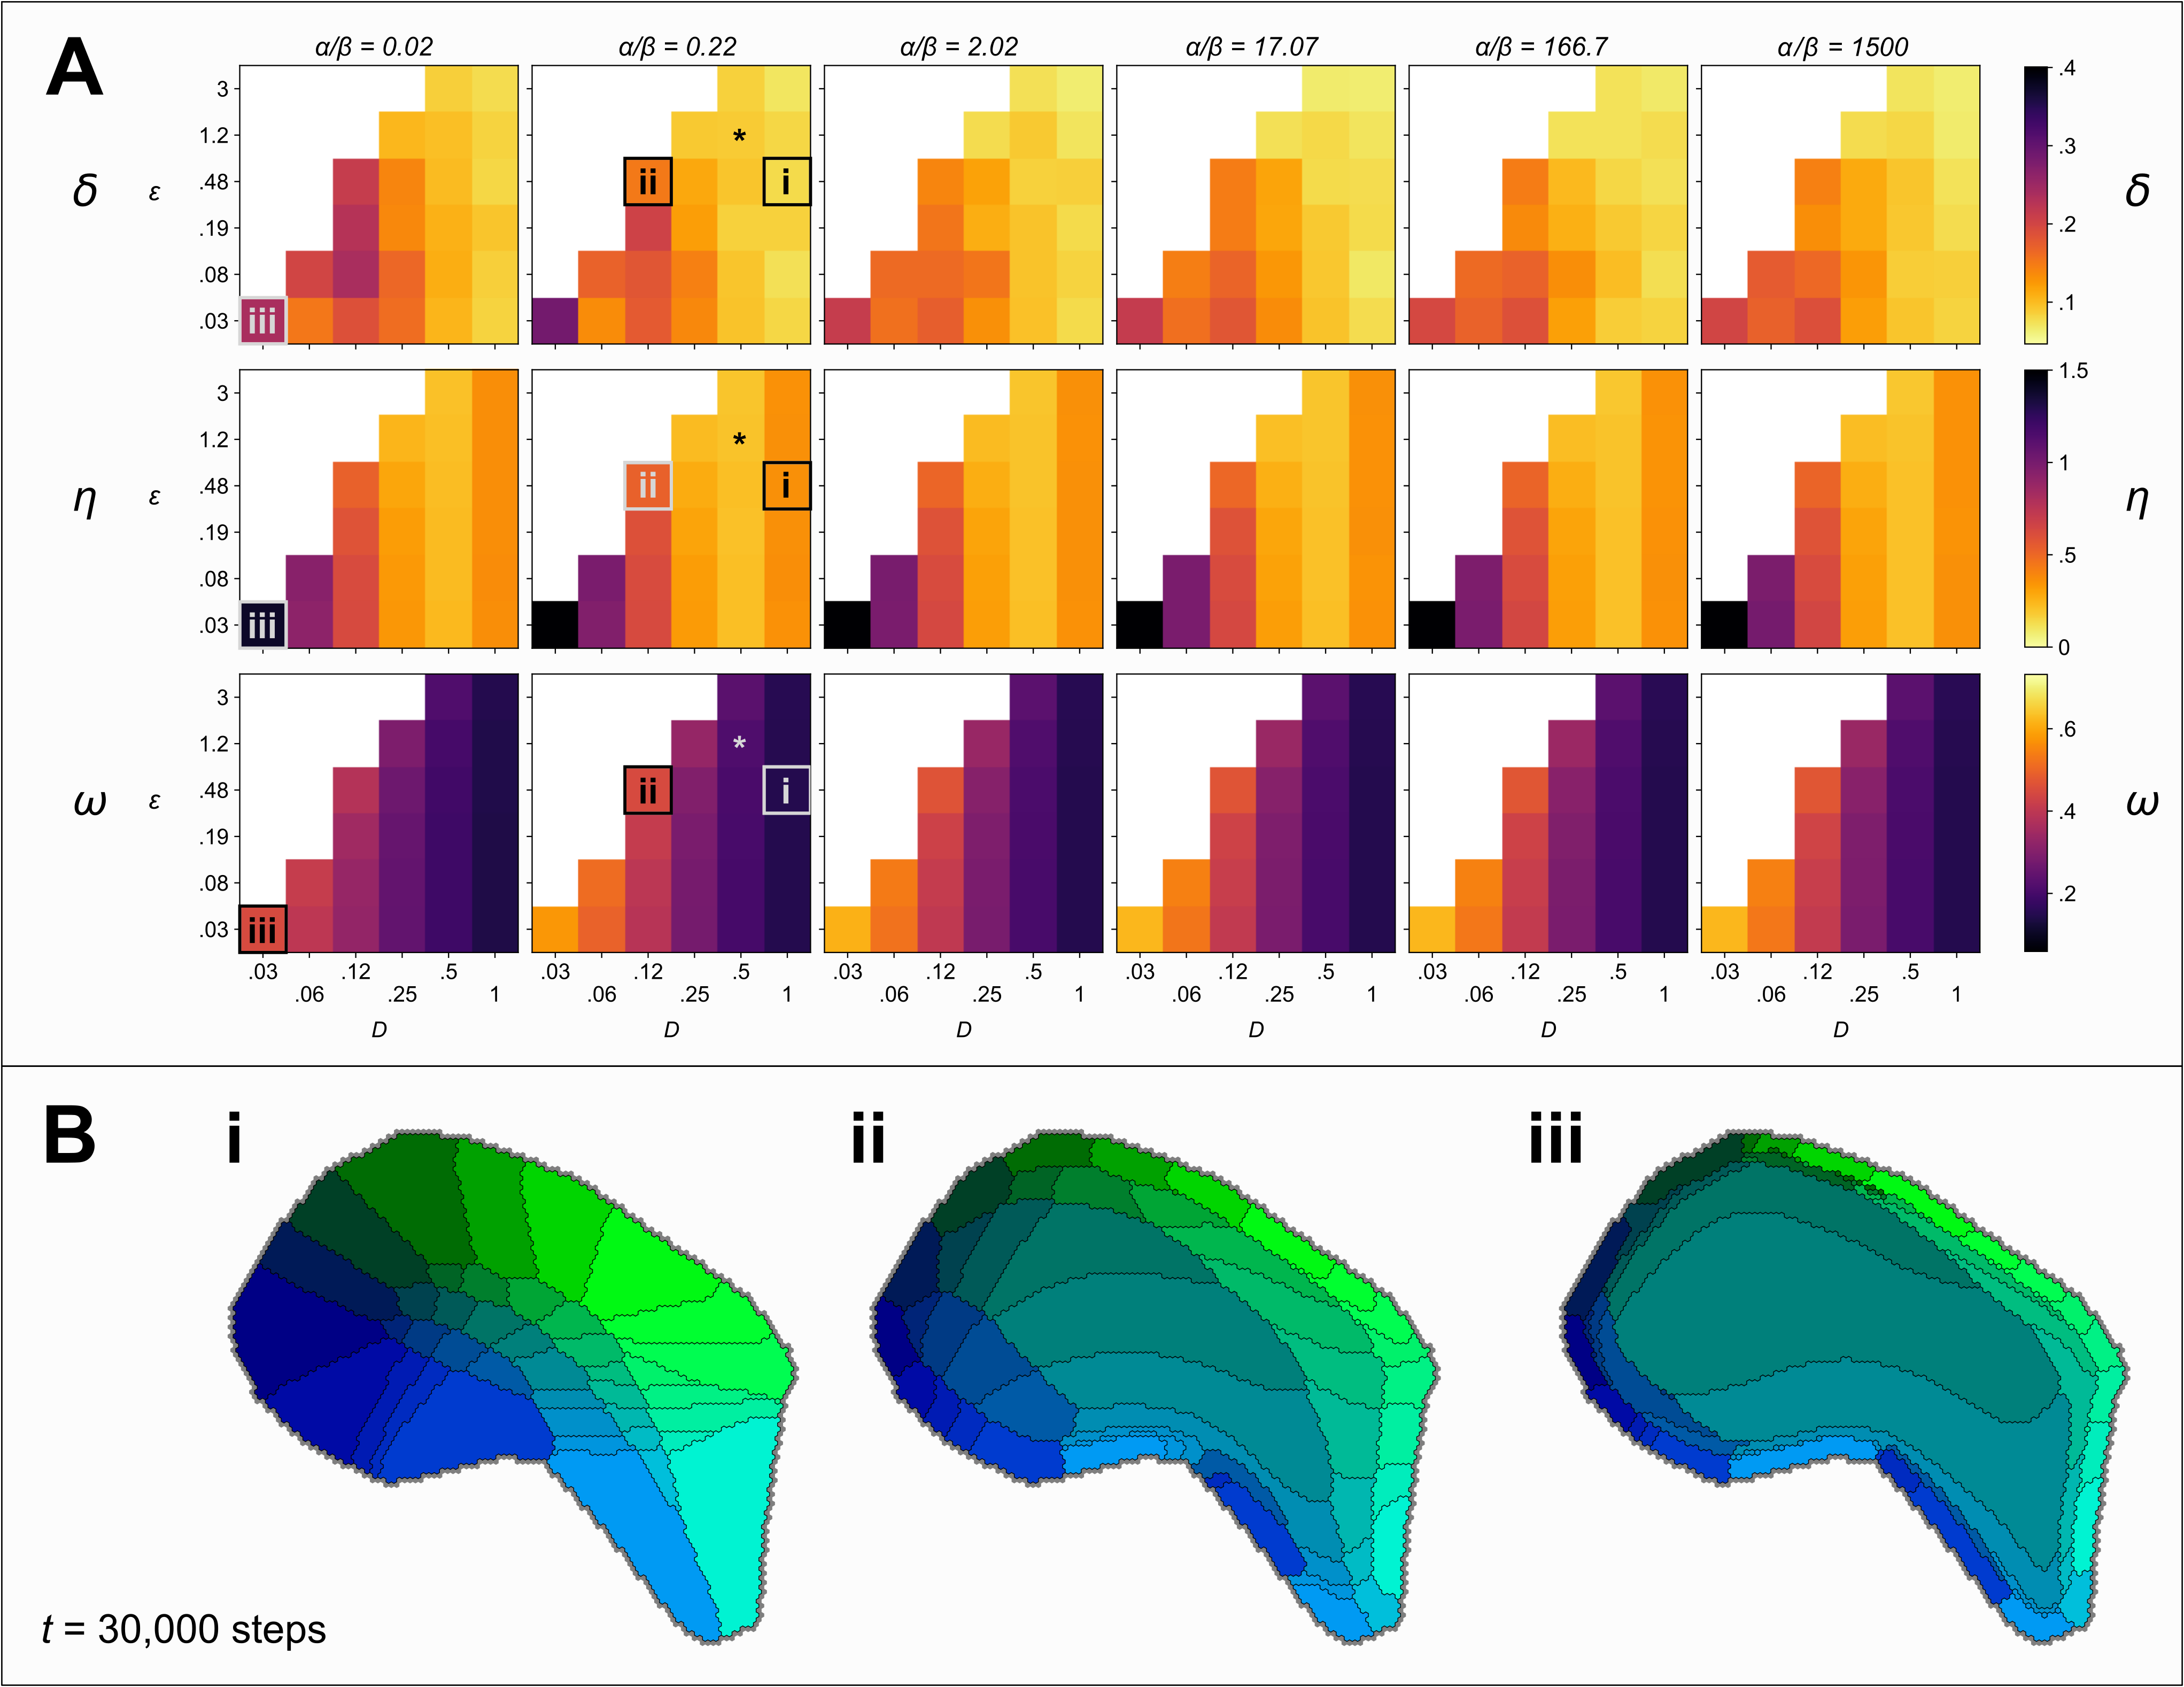
\includegraphics[width=\linewidth]{./Fig2.png}
    \caption{\MPthreePar{\textbf{A} Exploring the parameter space of the
        model given in Eqs.\,\ref{eq:dc}--\ref{eq:comp}. Graphs show the three
        pattern metrics for $t=30000$ steps as colourmaps: Honda $\delta$ (top
        row) shows conformance to a Voronoi pattern; $\eta$ (middle row) gives
        the simulated/experimental barrel area difference and $\omega$ (bottom
        row) is a measure of selectivity of the connection densities for the
        41 thalamocortical axon types. The colour maps are chosen so that for
        each row, lighter (orange and yellow) colours indicate desirable
        properties for the simulations: Lower values of $\delta$ are yellow,
        indicating good Voroni patterns; Lower values of $\eta$ indicate good
        pattern matching; Higher values of $\omega$ indicate greater
        selectivity. White squares indicate that the simulation was not stable
        for that parameter set.
%
        The parameter space explored is three dimensional with the parameter
        ratio $\alpha/\beta$ varied along the columns of graphs, the
        competition parameter $\epsilon$ varied on the $y$-axes and the
        diffusion constant, $D$ varied along the $x$-axes. An asterisk (*)
        marks the parameter set displayed in Fig.\,\ref{fig:main}. Boxes i),
        ii)~and iii)~mark parameter sets for which corresponding patterns are
        shown in \textbf{B} (for $t=30000$ steps).
%
        \textbf{B} The effect of varying the diffusion constant,
        $D$. i)~Increasing $D$ above the optimum value gives an expansion of
        the outer barrels and a corresponding compression of the barrels
        within. ii)~Conversely, an expansion of the central barrels and
        compression of those near the boundary results from reducing $D$ from
        its optimum. iii) Reducing the diffusion constant is equivalent to
        increasing the size of the domain $S$ and so this simulation, in which
        $D$ had the lowest stable value, can be thought to represent an animal
        with a large cortical area but with unchanged cortical complexity. A
        large proportion of the domain is occupied by the projections with
        intermediate interaction parameters; those with strong interaction
        parameters are compressed around the edge of the domain. A barrel
        pattern fails to form.}}
    \label{fig:paramsweep}
  \end{fullwidth}
\end{figure}

\MPthreePar{Fig.\,\ref{fig:paramsweep}A shows values of $\delta$, $\eta$ and
  $\omega$ obtained after 30000 iterations, from 216 independent simulations,
  each representing a unique combination of the model parameters $D$,
  $\epsilon$, and the ratio $\alpha/\beta$. First we observe that
  self-organization is highly robust to the ratio $\alpha/\beta$, across five
  orders of magnitude, with respect to all three metrics. Second, the most
  strongly Dirichletform patterns (low \emph{Honda}-$\delta$) were generated
  by simulations in which the diffusion constant $D$ and the strength of
  competition $\epsilon$ were high. Third, strongest connection selectivities,
  $\omega$, were obtained for lower values of $D$. Fourth, variation in the
  pattern difference metric, $\eta$, indicated that the alignment between real
  and simulated patterns was greatest for intermediate rates of diffusion,
  $D\approx0.5$. Together these results indicate that when competition is
  strong, the rate of diffusion determines a trade-off such that fields emerge
  to be barrel-shaped when diffusion is fast and they emerge to be more
  selectively innervated when diffusion is slow.}

\MPthreePar{The parameters of the example simulation are indicated in
  Fig.\,\ref{fig:paramsweep}A using an asterisk. In
  Fig.\,\ref{fig:paramsweep}B, we also present examples of alternative
  patterns that emerge for different choices of $D$. Decreasing the rate of
  diffusion may be considered equivalent to increasing the overall size of the
  domain, $S$, hence insights into barrel development in species with
  substantially larger barrel fields, such as capybara which do not have
  clearly identifiable barrels, may be gained by studying pattern formation
  when $D$ is small. In this context, it is interesting to note that for small
  $D$, the organization is predicted to be topological but highly irregular,
  with a general expansion in the territory occupied by the central versus
  peripheral domains that would presumably manifest as an absence of
  identifiable barrel fields (Fig.\,\ref{fig:paramsweep}B\,iii).}

% Full page width
\begin{figure}
  \begin{fullwidth}
    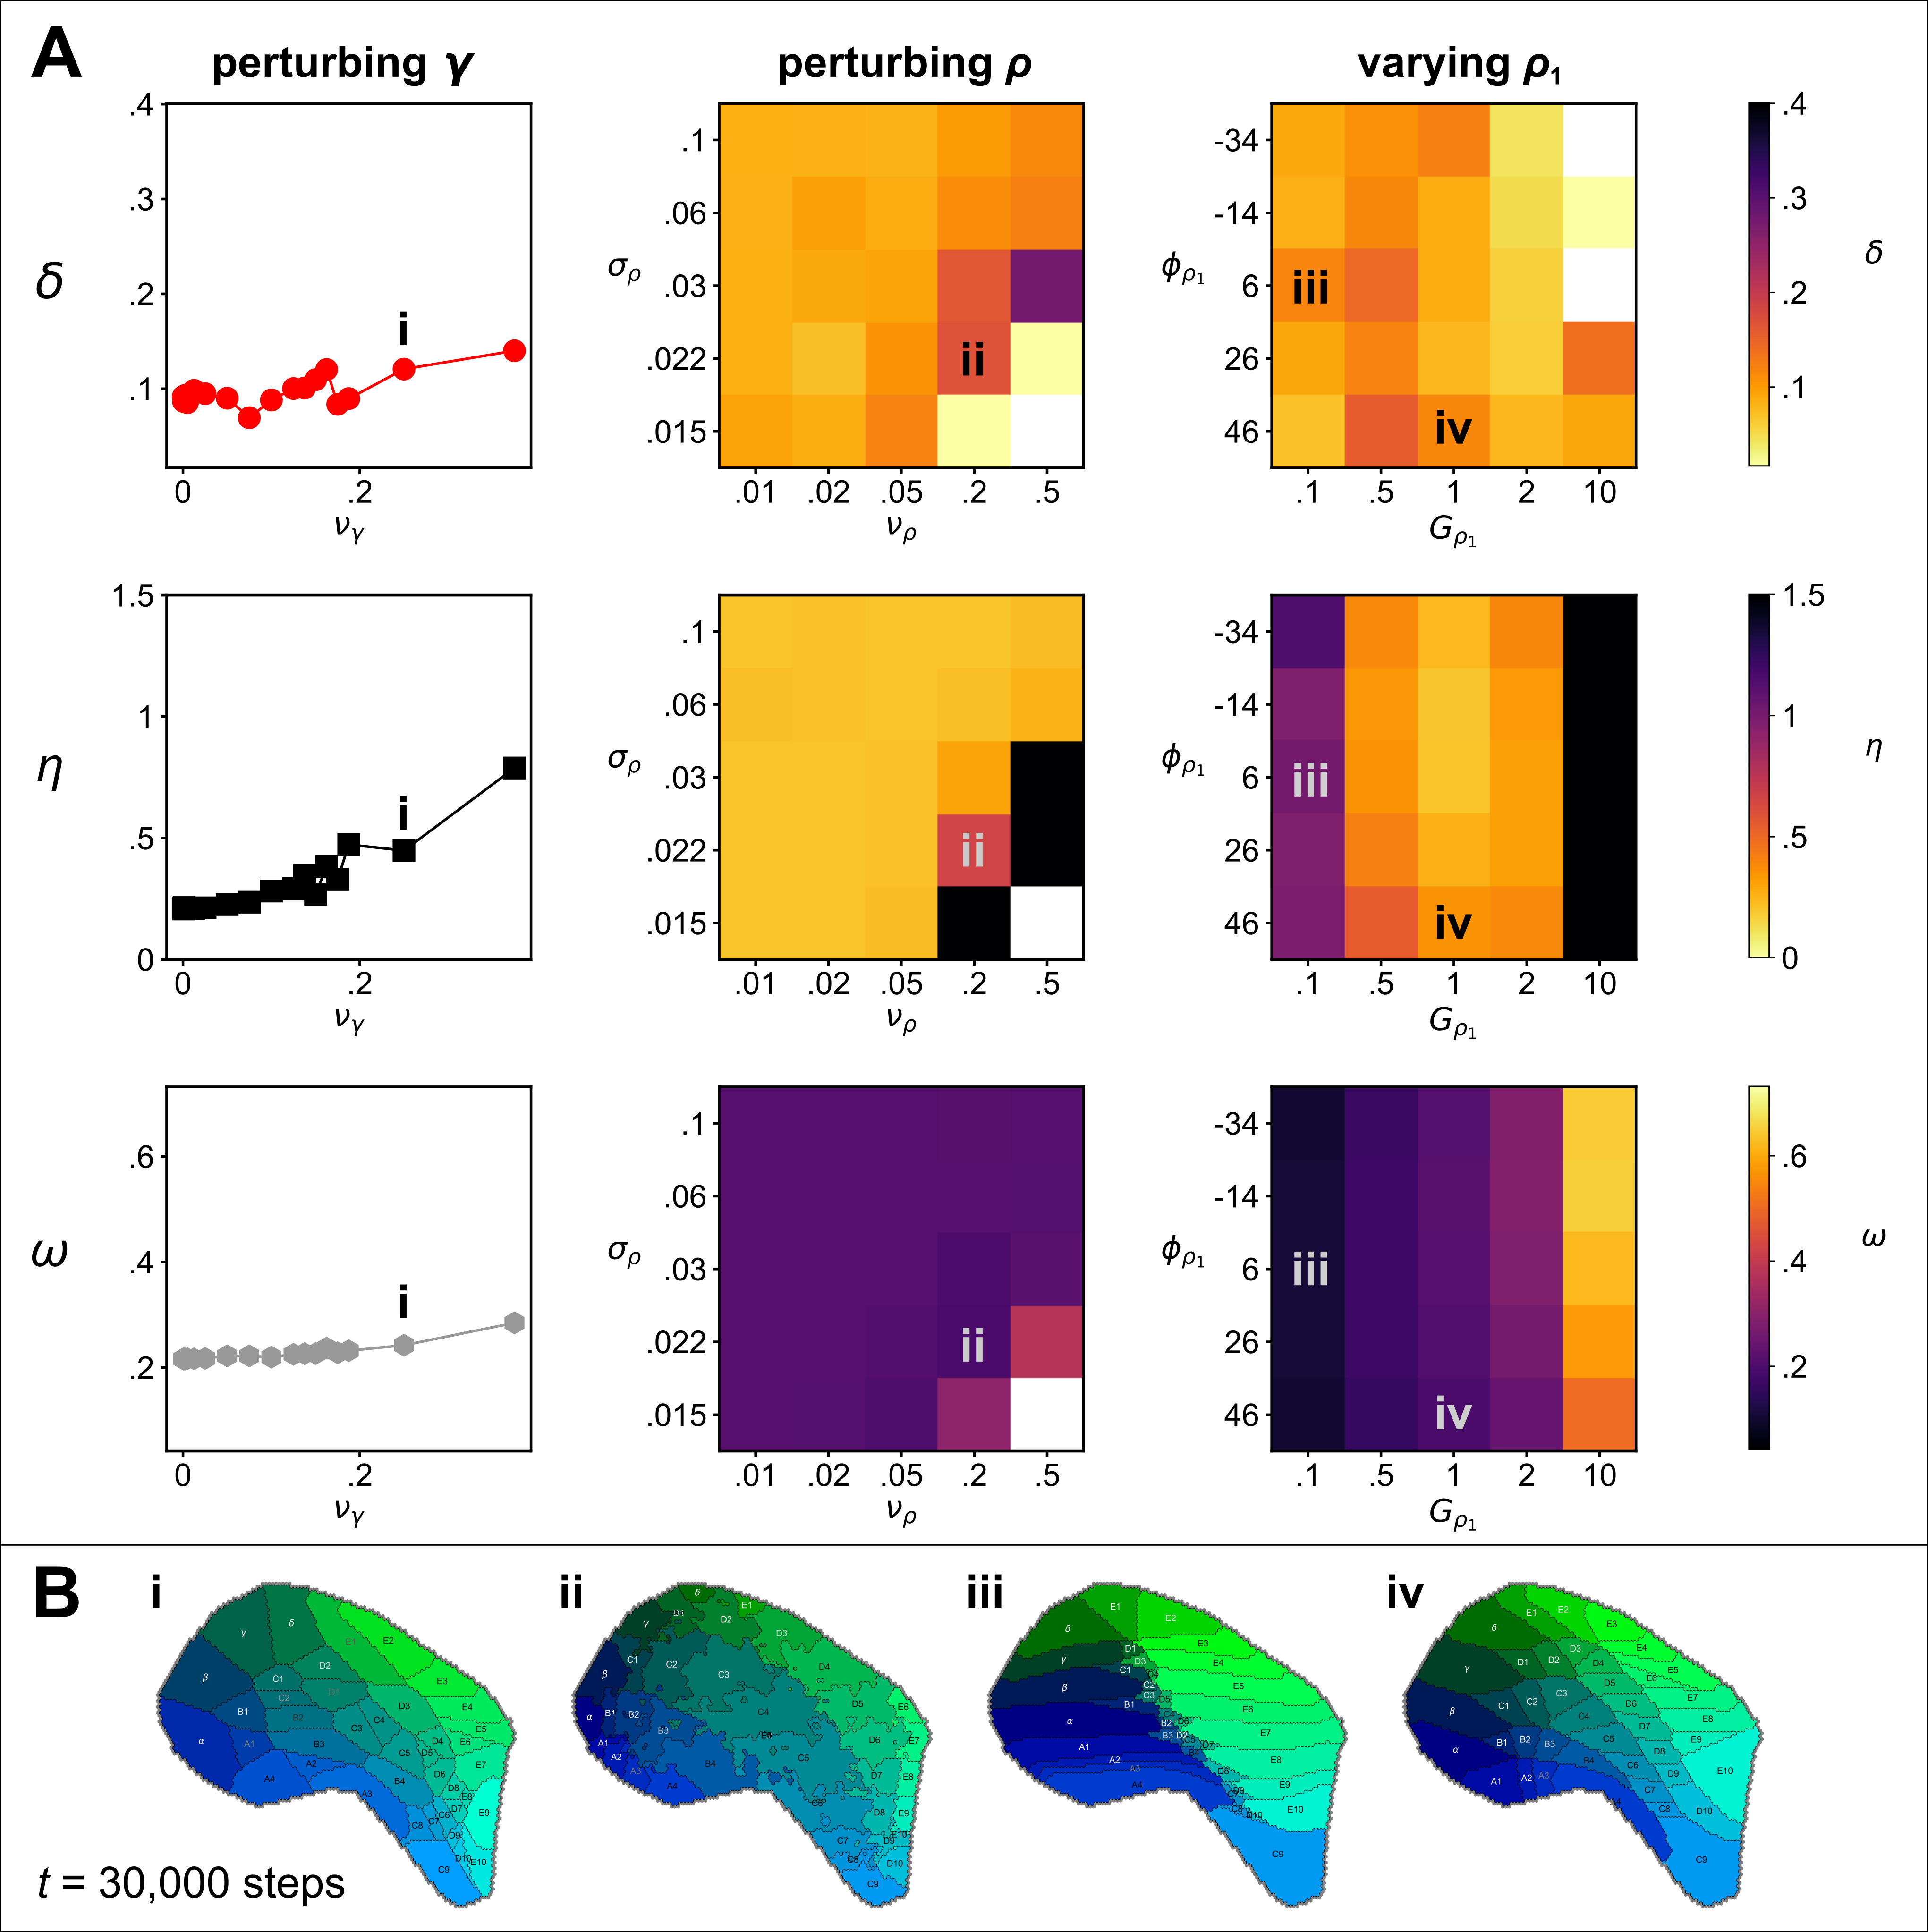
\includegraphics[width=\linewidth]{./Fig3.png}
    \caption{
      \MPthreeSens{\textbf{A} Sensitivity of the system pattern
        metrics $\delta(t)$ (top row), $\omega(t)$ (middle row) and $\eta(t)$
        (bottom row), evaluated at $t=30000$ steps,
        to three classes of perturbation. $y$-axes and colour scales have identical ranges
        to the colour scales in Fig.\,\ref{fig:paramsweep}, to ease comparison
        with the parameter exploration.
        %
        \emph{Column 1:} Random noise drawn from a uniform distribution,
        $(\gamma_{max}-\gamma_{min})\,U(0,\nu_\gamma)$, added
        to the values for the interaction parameters, $\gamma_{i,j}$ used in
        Fig.\,\ref{fig:main}.
        %
        \emph{Column 2:} Random noise $(\rho_{max} - \rho_{min})\,U(0, \nu_{\rho})$
        was added to each hex element of $\rho_1(\mb{x})$ and $\rho_2(\mb{x})$ and the result
        was smoothed by convolution with a symmetric 2D
        Gaussian kernel of width $\sigma_\rho$. Colour maps in this column
        thus show the effect of changing the magnitude and the length scale of
        noise in the guidance fields.
        %
        \emph{Column 3:} Colour maps show the result of setting the rotational angle
        of the linearly varying guidance field, $\rho_1(\mb{x})$, to $\phi_{\rho_1}$,
        and modifying its overall gain to $G_{\rho_1}$, whilst keeping the
        parameters of $\rho_2(\mb{x})$
        unchanged from those used in the simulation in
        Fig.\,\ref{fig:main}, for which
        $\phi_{\rho_2}=84$\textdegree and $G_{\rho_2}=1$.
        %
        \textbf{B} Four ways in which the perturbations in \textbf{A} affect
        the patterns. i) The effect of significant interaction parameter noise
        causes barrels to become swapped from the positions they would
        otherwise take. ii) High magnitude, short lengthscale noise in
        $\rho(\mb{x})$ leads to `wiggly' boundaries between barrels. iii)
        Shows the effect of reducing the slope of $\rho_1$ (by a factor of 10)
        which reduces the strength of the axons' interaction with the guidance
        field in the left-right sense. Barrel rows B, C and D become `crushed'
        down the center line, and edge barrels dominate. iv) The effect of
        rotating $\rho_1$ by 20\textdegree~is a relatively mild distortion of
        the pattern in the anticlockwise sense.
      }
    }
    \label{fig:sens}
  \end{fullwidth}
\end{figure}


\MPthreeSens{Next we conducted a sensitivity analysis to determine the extent
  to which the quality of the pattern (after $t=30000$ iterations) is affected
  by perturbations to i)~the magnitude and offset of the noise applied to
  $a_i$ at $t=0$; ii)~noise applied to the interaction parameters,
  $\gamma_{i,j}$; iii)~noise (at various length scales) applied to the
  guidance fields; and iv)~the magnitude and orientation of one cortical
  guidance field relative to the other (Fig.\,\ref{fig:main}A).}

\MPthreeSens{Using the parameters of the example simulation
  (Fig.\,\ref{fig:main}C) we established baseline mean and standard deviations
  from ten independent simulations with initial uniform random values for
  $a(\mb{x},0)\in(0.2,0.4)$, to be $\delta=0.089\pm 0.004$, $\eta=0.2108\pm
  0.002$, and $\omega=0.2165\pm 0.0001$. Repeating with the variation in the
  initial noise doubled ($a(\mb{x},0)\in(0.1,0.5)$), or removed altogether
  ($a(\mb{x},0)=0.3$), generated distributions of $\delta$, $\eta$, and
  $\omega$ that were not statistically different, as established using paired
  two-sample t-tests. Adding noise to the interaction parameters ($\gamma$)
  affected neither the \emph{Honda-}$\delta$ or the \emph{connection
    selectivity} measures substantially (see Fig.\,\ref{fig:sens}A), and an
  increase in the \emph{pattern difference} reflected an increase in the
  occurrence of topological defects only when perturbations become so large as
  to cause the ordering of $\gamma$ values from neighbouring thalamic sites to
  be switched (see example map Fig.\,\ref{fig:sens}B\,i). Adding noise to the
  cortical guidance field values, $\rho_1(\mathbf{x})$ and
  $\rho_2(\mathbf{x})$, disrupted pattern formation only for high levels of
  noise applied at short length scales, which manifested as non-straight edges
  at the domain boundaries (Fig.\,\ref{fig:sens}B\,ii). Varying the slope of one
  linear gradient $\rho_1(\mathbf{x})$ while keeping that of the other
  constant caused elongation of the emergent domains along the corresponding
  axis (Fig.\,\ref{fig:sens}B\,iii), while pattern formation was not strongly
  influenced by relaxing the assumption that the gradients of the two cortical
  guidance fields are orthogonal (Fig.\,\ref{fig:sens}B\,iv). Overall, the
  sensitivity analysis revealed that self-organization of barrel-like fields
  in the model is highly robust to a wide range of sources of perturbation.}

\MPthreePred{To further investigate the interplay of genetic and intrinsic
  mechanisms we simulated two well known experimental manipulations of the
  whisker barrel system. First, we simulated a seminal barrel duplication
  experimental paradigm}
\citep{shimogori_fibroblast_2005,assimacopoulos_fibroblast_2012}
\MPthreePred{in which the growth factor Fgf8, which is normally expressed at
  the anterior end of the cortical subplate from around E9.5}
\citep{crossley_mouse_1995}, \MPthreePred{is ectopically expressed (by
  electroporation) also at the posterior pole of a cortical
  hemisphere. Because Fgf8 sets off a chain of gene interactions involved in
  controlling the graded expression of ephrin and cadherin molecules, its
  misexpression at the posterior pole could be expected to mirror those
  gradients which usually vary along the rostrocaudal axis. We assume that
  this results in a mirror of the primary barrel cortex boundary along the
  rostrocaudal axis, to match the experimental results of}
\cite{assimacopoulos_fibroblast_2012}. \MPthreePred{We also assume that a
  further consequence of the posterior Fgf8 electroporation is the mirrored
  anterior-posterior guidance gradient $\rho_1$ (Fig.\,\ref{fig:fgf8}A). With
  the modified $\rho_1$ guidance gradient the simulation was run with $N=41$
  thalamocortical axon types, using the parameters of the example
  simulation. The result, after 30000 iterations, was two mirror-symmetrical
  barrel fields comprising $2N$ barrels (Fig.\,\ref{fig:fgf8}B), consistent
  with the outcome of the original experiments.}

% This figure is text width
\begin{center}
  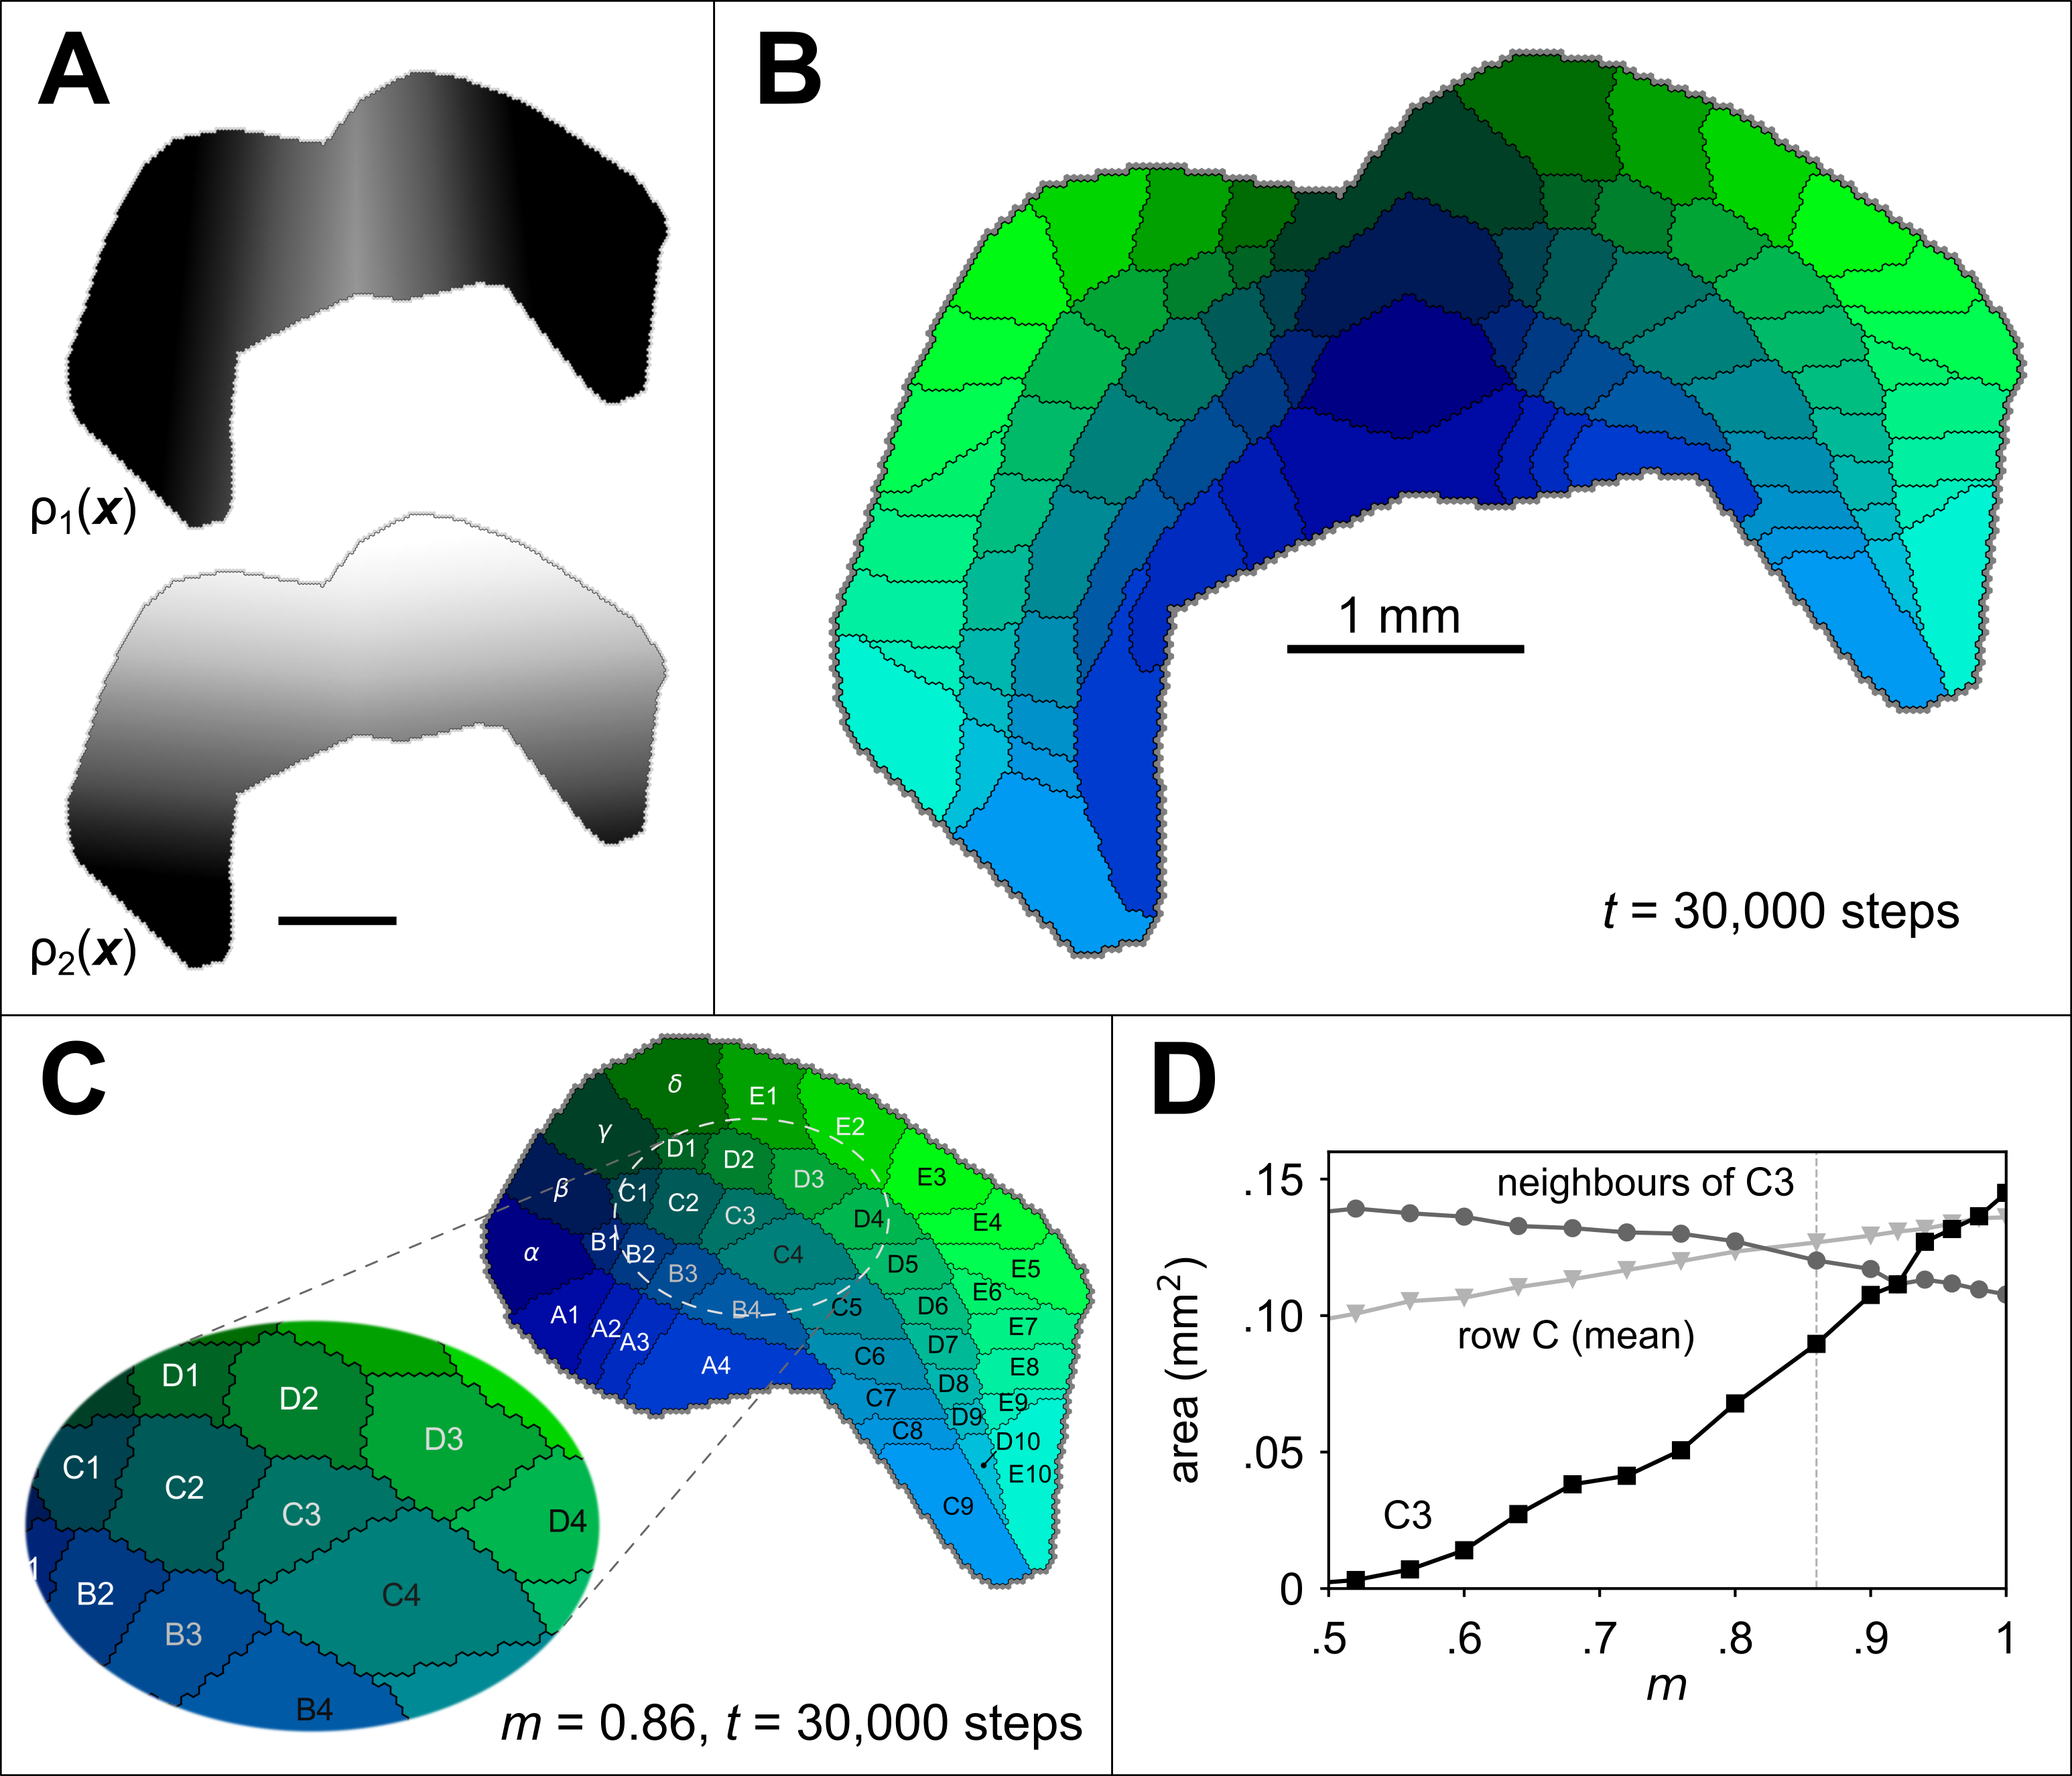
\includegraphics[width=\linewidth]{./Fig4.png} \captionof{figure}{
    \MPthreePred{Two simulated whisker barrel manipulations.  Guidance fields
      (\textbf{A}) and emergent barrel pattern (\textbf{B}) in a Fgf8
      misexpression experiment
      (c.f.~\citealp{assimacopoulos_fibroblast_2012}), simulated by reflecting
      $\rho_1$ from Fig.\,\ref{fig:main}A at the join of the original boundary
      with its mirror. The model parameters match those in
      Fig.\,\ref{fig:main}C.  Scale bars are 1\,mm. \textbf{C} Simulating
      whisker trimming by a reduction of the competition parameter,
      $\epsilon$, in the expression $\chi_i$ (Eq.\,\ref{eq:comp}) for the C3
      thalamocortical projection. For C3, $\epsilon$ is replaced by
      $m\,\epsilon$, where $m$ is a scalar multiplier. For the rest of the
      projections, $\chi_i$ is left unchanged and all other parameters are
      identical to those reported in Fig.\,\ref{fig:main}C. The pattern formed
      after 30000 steps with $m=0.86$. As its axon branching competes weakly
      with its neighbours, field C3 is reduced to 65\% of its original size,
      matching the average barrel area reduction observed by }
    \citealp{kossut_effects_1992}. \MPthreePred{\textbf{D} Individual barrel
      area (mm$^2$) plotted vs.~$m$ for C3 (black squares) shows that as $m$
      is reduced, its area goes down, disappearing for $m\approx0.5$, whereas
      the mean area of neighbouring barrels B3, C2, C4, D2 \& D3 (grey
      circles) increases. The dotted grey line indicates $m=0.86$ for
      comparison with panel C.}}
  \label{fig:fgf8}
\end{center}

\MPthreePred{To investigate the response of the model to environmental
  manipulation, we simulated a whisker deprivation experiment. In the first
  few days after birth, the upper region of the rat's cortex develops into
  distinct layers I--IV (layers V and VI are already distinct at
  birth). During this critical period, removal of the mystacial whiskers by
  electrocauterization, plucking or trimming leads to observable changes in
  brain structures, including the barrel field in cortical layer
  IV~\citep{jeanmonod_mouse_1981}. Amoungst other changes, barrels associated
  with deprived whiskers have a smaller area. This is found whether the animal
  is deprived of an individual whisker~\citep{kossut_effects_1992}, or an
  entire row~\citep{loos_somatosensory_1973}, and demonstrates that
  thalamocortical activity contributes to the developmental process. We
  simulated the trimming of the individual whisker C3 during this critical
  period by reducing the amount by which its thalamocortical projections
  compete for branching. This was achieved by reducing the value of $\epsilon$
  in Eq.\,\ref{eq:comp} for the C3 projection, leaving other simulation
  parameters unchanged. The reduced competition for branching limited the area
  over which the C3 projection could make connections and its resulting field
  size was diminished (Fig.\,\ref{fig:fgf8}C). Emergent fields representing
  the neighbours of the C3 projection, whose ability to compete for branching
  was unchanged, increased in size. The C3 barrel disappeared altogether if
  its competition parameter was reduced below a half of the original value. A
  reduction in the area of barrel C3, comparable that induced by
  \citealp{kossut_effects_1992} (65\%) was obtained in simulation when the
  competitiveness of projection C3, $\epsilon$, was reduced to 86\%, as
  indicated in Fig.\,\ref{fig:fgf8}D.}

\MPthreePred{Together with the results of the misexpression experiment, the
  consistency of the simulated whisker trimming results with those of the
  original studies demonstrates how the model can be used to test specific
  hypotheses about the contribution of intrinsic and extrinsic factors to the
  development of cortical fields.}

\section{Discussion}

The present results suggest that the key requirements for the emergence of
realistic barrel patterning are i)~at each cortical location thalamocortical
projections compete for a limited number of available synaptic connections
(Eqs.~\ref{eq:dc}--\ref{eq:da}), ii)~at each location the branching rate of a
given projection is reduced by the density of other projections
(Eq.\,\ref{eq:comp}), and iii)~the branch density of each projection is
conserved over time.

The emergence of barrels in simulation required competition between thalamic
projections in terms of synaptic connectivity and also competition in terms of
cortical space, as represented by $\chi$, with an implicit requirement for a
self/other identifier amoungst projections. This latter form of competition may account for the absence of barrels in rodents with larger brains, such as
capybara, for which competition for space is presumably weaker
\citep{woolsey_comparative_1975}. Hence, irrespective of whether barrels are
necessary for adaptive whisker function, the emergence of somatotopically
ordered modular structures may be an inevitable consequence of local
competition for cortical territory driven by input from an array of discrete
sensory organs \citep{purves_iterated_1992}.

\cmnt{In reality, scores of smaller Dirichletform barrels representing the
  microvibrissae form to the right of where the E-row barrels emerge in our
  simulations, presumably via the same competitive processes. Enforcing here
  the same boundary condition as used to represent the true edges of the
  barrel field is necessary to ensure the stability of the simulation, though
  we acknowledge that this region of the boundary is enforced primarily to
  keep the number of simulated projections, and hence the overall
  computational complexity of the simulation, manageable (simulating each
  additional projection introduces an extra 13030 new dynamical
  variables).}

It is important to emphasize that the formulation of the model is entirely
local, insofar as simulation requires no information to be communicated from a
given cortical grid cell to any but those immediately adjacent (via
diffusion). Hence the simulations demonstrate how a self-organizing system,
constrained by genetically specified guidance cues and by the shape of the
cortical field boundary, can faithfully reproduce an arrangement of cell
aggregates in one neural structure as a topographic map in another.

Moreover, the present results confirm that somatotopic map formation does not
require the pre-specification of center-points by as yet undetermined
additional developmental mechanisms.

\section{Materials \& Methods}

% Be sure to include/mention:
%
% The no-flux boundary conditions applied in the \cite{karbowski_model_2004}
% model are retained.
%
% Arbitrary boundary shapes were applied

The cortical sheet was modelled as a two dimensional hexagonal lattice, which
simplifies the computation of the 2D Laplacian. Within a boundary traced
around the edge of a
rat barrel field (Fig.\,\ref{fig:main}A) we set the hex-to-hex distance
$d$ to 0.03\,mm, which resulted in a lattice containing 6515 hexes for the
simulations shown in Figs.\,\ref{fig:main}A,C \& D and 12739 hexes for the Fgf8
misexpression study shown in Fig.\,\ref{fig:fgf8}. Each hex contained 82 time-dependent
variables: 41 branching densities ($a_i$) and 41 connection densities ($c_i$).
The rate of change of each of the time-dependent variables (Eqs.\,\ref{eq:dc}
\& \ref{eq:da}) was computed using a fourth-order Runge-Kutta method.

The most involved part of this computation is to find the divergence of the
flux of axonal branching, $\mb{J}_i(\mb{x},t)$, the term in parentheses in
Eq.\,\ref{eq:da}:
%
\begin{equation}
  \label{eq:divJ}
  \nabla\vcdot\mb{J}_i(\mb{x},t) = \nabla\vcdot\left(D \nabla
  a_i-a_i\sum_{j=1}^{M} \gamma_{i,j}\nabla \rho_j(\mb{x}) \color{colmptwo}+
  \frac{\epsilon a_i}{N-1} \nabla \hat{a}_i \color{black}\right),
\end{equation}
%
\MPtwo{where $\hat{a}_i\equiv\sum_{j\ne i}^{N}a_j$.} Note that the sum of the
guidance gradients is time-independent and define $\mb{g}_i(\mb{x}) \equiv
\sum_{j=1}^{M} \gamma_{i,j} \nabla\rho_j(\mb{x})$.  Because the divergence
operator is distributive, Eq.\,\ref{eq:divJ} can be expanded using vector
calculus identities (dropping references to $\mb{x}$ and $t$ for clarity):
%
\begin{equation}
\nabla\vcdot\mb{J}_i = \nabla\vcdot\big(D \nabla a_i\big) -
\nabla\vcdot\big(a_i \mb{g}_i\big) \color{colmptwo} + \frac{\epsilon}{N-1}\nabla\vcdot\big({a}_i\nabla\hat{a}_i\big)\color{black}.
\end{equation}
%
Applying the vector calculus product rule identity yields
%
\begin{equation} \label{eq:divJExpanded}
%
\nabla\vcdot\mb{J}_i =
%
D \dvrg a_i % term1
-
a_i\nabla\vcdot\mb{g}_i % term2
-
\mb{g}_i\vcdot\nabla a_i % term3
\color{colmptwo}
+ \frac{\epsilon a_i}{N-1} \dvrg \hat{a}_i % term1_1
+ \frac{\epsilon}{N-1} \nabla \hat{a}_i\vcdot\nabla{a}_i% term1_2
\color{black}
,
\end{equation}
%
which has \MPtwo{five} elements to compute: i)~$D \dvrg a_i$ (the Laplacian of
$a_i$); ii)~a time-independent modulator of $a_i$ (because
$\nabla\vcdot\mb{g}_i$ is a time-independent static field); iii)~the scalar
product of the static vector field $\mb{g}_i$ and the gradient of $a_i$;
\MPtwo{iv)~the Laplacian of $\hat{a}_i$; and v)~a term involving the gradients
  of $a_i$ and $\hat{a}_i$}. Each of the divergences can be simplified by
means of Gauss's Theorem following \cite{lee_hexagonal_2014}.

(i) The computation of the mean value of the Laplacian across one hexagon of
area $\Omega = \frac{\sqrt{3}}{2}d^2$, located at position $\mb{p}_0$, with
neighbours at positions $\mb{p}_1$--$\mb{p}_6$ is
%
\begin{equation} \label{eq:lapl}
\begin{split}
\langle D \dvrg a_i(\mb{p}_0,t) \rangle  = \frac{D}{\Omega} \oiint_\Omega \dvrg a_i(\mb{x}, t) \dif\Omega & = \frac{D}{\Omega} \oint \frac{\partial a_i}{\partial \hat{\mb{n}}} \dif\gamma \\
& \approx \frac{D}{\Omega} \sum_{j=1}^6 \frac{\partial a_i(\mb{p}_j)}{\partial \hat{\mb{n}}} \bigg\rvert_{\mathrm{mid}} v \\
& = \frac{2D}{\sqrt{3} d^2} \sum_{j=1}^6 \frac{a_i(\mb{p}_j) - a_i(\mb{p}_0)}{d} \frac{d}{\sqrt{3}} \\
& = \frac{2D}{3 d^2} \sum_{j=1}^6 \big(a_i(\mb{p}_j) - a_i(\mb{p}_0)\big),
\end{split}
\end{equation}
%
where $v = d/\sqrt{3}$ is the length of each edge of the hexagon and $\dif\gamma$
is an infinitesimally small distance along its perimeter.

\noindent
ii) The computation of the second term in Eq.\,\ref{eq:divJExpanded},
$\langle a_i(\mb{p}_0,t)\nabla\vcdot\mb{g}_i(\mb{p}_0)\rangle$, can be written out similarly:

\begin{equation} \label{eq:divg}
\begin{split}
%
\frac{1}{\Omega} \oiint_\Omega a_i\nabla\vcdot\mb{g}_i\;\dif\Omega & = \frac{a_i(\mb{p}_0,t)}{\Omega}  \oint \mb{g}_i\vcdot \dif\hat{\mathbf{n}} \\
%
& \approx \frac{a_i(\mb{p}_0,t)}{\Omega} \sum_{j=1}^{6} \frac{\mb{g}_i(\mb{p}_j) + \mb{g}_i(\mb{p}_0)}{2}\vcdot \hat{\mb{n}}\;v \\
%
& = \frac{2 a_i(\mb{p}_0,t)v}{\sqrt{3}d^2} \sum_{j=1}^{6} \bigg[ \frac{g_i^x(\mb{p}_j) + g_i^x(\mb{p}_0)}{2} \vcdot  \hat{\mb{n}} + \frac{g_i^y(\mb{p}_j) + g_i^y(\mb{p}_0)}{2} \vcdot  \hat{\mb{n}} \bigg] \\
%
%%& = \frac{2 a_i(\mb{p}_0,t)d}{\sqrt{3}d^2\sqrt{3}} \bigg( \sum_{j=1}^{6} \frac{\mb{g}_j^x + \mb{g}_0^x}{2} \vcdot  \hat{\mb{n}} + \sum_{j=1}^{6} \frac{\mb{g}_j^y + \mb{g}_0^y}{2} \vcdot  \hat{\mb{n}} \bigg) \\
%
%\Rightarrow \langle a_i(\mb{p}_0,t)\nabla\vcdot\mb{g}(\mb{p}_0)\rangle &
%\approx \frac{a_i(\mb{p}_0,t)}{3d} \bigg( \sum_{j=1}^{6} \big(g_i^x(\mb{p}_j)
%+ g_i^x(\mb{p}_0)\big) \cos \big(\frac{\pi}{3}(j-1)\big) + \sum_{j=1}^{6}
%\big({g_i^y(\mb{p}_j) + g_i^y(\mb{p}_0)}\big) \sin
%\big(\frac{\pi}{3}(j-1)\big) \bigg), \\
%% Condensing into a single sum:
\Rightarrow \langle a_i(\mb{p}_0,t)\nabla\vcdot\mb{g}(\mb{p}_0)\rangle & \approx \frac{a_i(\mb{p}_0,t)}{3d} \sum_{j=1}^{6} \bigg[ \big(g_i^x(\mb{p}_j) + g_i^x(\mb{p}_0)\big) \cos \big(\frac{\pi}{3}(j-1)\big) + \big({g_i^y(\mb{p}_j) + g_i^y(\mb{p}_0)}\big) \sin \big(\frac{\pi}{3}(j-1)\big) \bigg], \\
%
\end{split}
\end{equation}
%
where $g_i^x$ and $g_i^y$ are the Cartesian components of $\mb{g}_i$. Both this
last expression, and the final expression of Eq.\,\ref{eq:lapl} can
be computed locally, by summing over values of the nearest neighbours.

\noindent
iii) The \MPtwo{middle} term in Eq.\,\ref{eq:divJExpanded} is the scalar product of two
vector fields which is straightforward to compute from their Cartesian
components.

\noindent
\MPtwo{iv) The same method used to compute $\dvrg a_i$ in term (i) is used to compute
$\dvrg \hat{a}_i$.}

\noindent
\MPtwo{v) The final term is the scalar product of the two vector fields $\nabla
  a_i$ and $\nabla \hat{a}_i$.}

By separating the computation of Eq.\,\ref{eq:divJ} into parts (i)--(v), the
no-flux boundary condition,
%
\begin{equation}
  \label{eq:noflux}
  \mb{J}_i(\mb{x},t)\big\rvert_{\mathrm{boundary}} = 0,
\end{equation}
%
can be fulfilled. On
the boundary, the contribution to $\mb{J}$ resulting from the first term of
Eq.\,\ref{eq:divJExpanded} can be fixed to 0 by the `ghost cell method' in
which, during the evaluation of (i), a hex outside the boundary containing the
same value as the hex inside the boundary is imagined to exist such that the
flux of $\mb{J}$ across the boundary is 0. Then, $\mb{g}_i(\mb{x})$ can be
tailored so that it, and its normal derivative approach 0 at the boundary,
ensuring that the second and third terms of Eq.\,\ref{eq:divJExpanded} also
contribute nothing to $\mb{J}$. This is achieved by \MPtwo{multiplying}
$\mb{g}_i(\mb{x})$ \MPtwo{by} a sharp logistic function of the distance, $d_b$,
from $\mb{x}$ to the boundary, \MPtwo{of the form $1/[1 +
  \exp(100(d_f-d_b))]$, where $d_f=0.1$\,mm is the boundary fall-off distance,
  chosen to be approximately $3d$}.

\metrics{The pattern-matching metric, $\eta$, incorporates information about i)
  the differences in the areas of the simulated and experimental barrels
  ($\mathcal{A}_i^{\mathrm{sim}}$ and $\mathcal{A}_i^{\mathrm{exp}}$); and ii)
  the information provided by `adjacency vectors', $\mathcal{V}_i$ (one for
  each barrel) whose $N$ elements contain the length of the barrel boundary
  which adjoins each other barrel in the pattern. The value of
  $\mathcal{V}_{i,j}$ (the $j^{\mathrm{th}}$ element of $\mathcal{V}_i$) is
  the length of the boundaries between regions of type $i$ and regions of type
  $j$. In a well-formed barrel pattern, $\mathcal{V}_{i}$ is a sparse vector
  and note that $\mathcal{V}_{i,i} = 0, \forall i$. $\mathcal{V}_{i}$ can be
  computed for the experimental and simulated barrel patterns and compared. A
  dimensionless measure of the pattern's arrangement and neighbour relations
  can be obtained from the scalar product of the simulated and experimental
  adjacency vectors:
  $\frac{1}{N} \sum_i \frac { \mathcal{V}_{i}^{\mathrm{sim}}}
  {b_{i}^{\mathrm{sim}} } \vcdot \frac{\mathcal{V}_{i}^{\mathrm{exp}}}{b_{i}^{\mathrm{exp}}}$, where
  $b_i^{\mathrm{exp}}$($b_i^{\mathrm{sim}}$) is the total length of the boundary of
  experimental(simulated) barrel $i$. This measure is low early in the simulation, when the regions do
  not have the neighbour relations of the experimental pattern
  (Fig.\,\ref{fig:main}C, $t=1000$) and maximal when the neighbour relations
  have become established ($t=10000$). It does not distinguish between
  $t=10000$ and $t=30000$.}
%
\metrics{A second way to analyse the adjacency vectors is to consider
  the mean magnitude of the difference between the simulated and experimental
  vectors: $\frac{1}{N} \sum_i \norm{ \mathcal{V}_{i}^{\mathrm{sim}} -
    \mathcal{V}_{i}^{\mathrm{exp}} } $. This tends to 0 for a perfect
  match and can separate patterns with straight boundaries from those with
  noise on the boundary shape (For an example of `noisy edges', see Fig.\,\ref{fig:sens}B\,ii).}
%
\metrics{We combined all of these measures into a single pattern quality metric:}
%
\begin{equation} \label{eq:eta}
\color{colmetrics}
  \eta =
  \frac
  {
    \frac{1}{N} \sum_i \norm[\big]{ \mathcal{A}_i^{\mathrm{sim}} - \mathcal{A}_i^{\mathrm{exp}} }
    \times
    \frac{1}{N} \sum_i \norm[\big]{ \mathcal{V}_{i}^{\mathrm{sim}} -
      \mathcal{V}_{i}^{\mathrm{exp}} }
  }
  {
    \frac{1}{N}
    \sum_i \frac {\mathcal{V}_{i}^{\mathrm{sim}}} {b_{i}^{\mathrm{sim}}}
    \vcdot
    \frac {\mathcal{V}_{i}^{\mathrm{exp}}} {b_{i}^{\mathrm{exp}}}
  },
\color{black}
\end{equation}
%
\metrics{which has units of mm$^3$.}

% for ``end of methods''
\MPone{We concentrated on the representation of the forty-six macrovibrissae
  that constitute a given barrel field, because their thalamic and cortical
  correlates are easily identifiable and consistently positioned. We exclude
  the representation of the microvibrissae to limit the overall complexity of
  the simulations, as well as the five rhinal whiskers as their representation
  in S1 is isolated from the main barrel field. Consequently, we set $N=41$.}

All code required to reproduce these results is available at
\url{https://github.com/ABRG-Models/BarrelEmerge/tree/eLife}. The computations
described in (i)--(v) may be found in the class method
\code{RD\_James\MPtwo{\_comp2}::compute\_divJ()} which calculates \code{term1},
\code{term2}, \code{term3}, \code{term1\_1} and \code{term1\_2}, respectively.

\section{Movie S1 caption}

Movie corresponding to Fig.\,\ref{fig:main}C in the main paper. Simulation parameters were
$N=41$, $\alpha=3.6$, $\beta=16.67$, $k=3$, $D=0.5$, $\gamma\in\pm 2$,
$\epsilon=1.2$ and $\delta{t}=0.0001$. Colours indicate the thalamic
projection for which the connection density is maximal, black lines delineate
boundaries, and overlaid contours show $c>0.5$. The final frame in the movie
is step 30000 of the simulation.

\section{Acknowledgments}

The authors thank Jason Berwick at the University of Sheffield for advice and
for access to the rat barrel stains used to construct Fig.\,1A. This work was
supported by a Collaborative Activity Award, \emph{Cortical Plasticity Within
  and Across Lifetimes}, from the James S.~McDonnell Foundation (grant
220020516).

\bibliography{../BarrelEmerge}

\end{document}
